\title[command line]{Command-line usage}
\author[Xuxin]{Xuxin Ma}
\institute[KAUST]{King Abdullah University of Science and Technology}
\date[Madagascar School 2011]{Beijing, Jul 21, 2011}

\begin{frame}
  \titlepage
\end{frame}

% \begin{frame}
%   \frametitle{Prerequisite}
  
%   \begin{itemize}
%   \item *NIX environment (UNIX, Linux, OS X, Cygwin, \ldots)
%   \item Shell (bash, csh, zsh, \ldots)
%   \item A working \textsc{Madagascar} 
%     % \item Editor (vi, emacs, \ldots)
%     % \item \LaTeX package ({\TeX}live, Mac{\TeX}, Mik{\TeX}, \ldots)
%     % \item Python $2.2$ to $2.7$
%   \end{itemize}
% \end{frame}
% \note{}

\begin{frame}
  \frametitle{Outline}
  \tableofcontents
\end{frame}

\section{\textsc{Madagascar}  Programs}

\begin{frame}
  \frametitle{\textsc{Madagascar} programs}
  
  \begin{itemize}
  \item ``sf'' prefix
  \item $812$ programs (2011-07-15)
  \item $30+$ developers
  \item Developed using C, C++, Fortran, Python
  \item Applications
    \begin{itemize}
    \item Numerical recipes
    \item General data analysis
    \item Seismic processing
    \item Visualization
%    \item Specific research purposes
    \end{itemize}
  \end{itemize}
\end{frame}
\note{in a recent subversion, there are over 7400 programs.
These programs are developed by a group of researchers.
m8r progs are developed using C, C++, etc
These progs cover a wide range of purposes.
}

\begin{frame}
  \frametitle{\textsc{Madagascar} programs}
  
  \begin{block}{List of all programs}
    \sh{sfdoc -k .} or \url{http://www.ahay.org/RSF}
  \end{block}
  \lstinputlisting[linerange=2-8]{sh.txt}

  \pause
  \begin{block}{Look for specific programs}
    \sh{sfdoc -k keyword}
  \end{block}
  \lstinputlisting[linerange=10-15]{sh.txt}
\end{frame}
\note{to count total n of progs: sfdoc -k . | wc -l}

\begin{frame}
  \frametitle{Self documentation}

  \begin{block}{Print out documentation}
    \sh{sfprog} without arguments
  \end{block}
  \lstinputlisting[linerange=17-32]{sh.txt}
\end{frame}

\begin{frame}
  \frametitle{Self documentation}
  
  \lstinputlisting[linerange=33-41]{sh.txt}
  
  \pause
  \begin{block}{}
    Computation examples under \textcolor{red}{\texttt{USED IN}} section
  \end{block}
  \lstinputlisting[linerange=43-51]{sh.txt}
\end{frame} 
\note{yet need to figure out how to highlight a word
}

\begin{frame}
  \frametitle{Command-line usage}

  \begin{block}{Single program}
    \sh{[< in.rsf] sfprog [par1=] [par2=] [...] [> out.rsf]}
  \end{block}
  \begin{itemize}
  \item Single input \texttt{< in.rsf}
  \item Single output \texttt{> out.rsf}
  \item Multiple parameters \texttt{par=val}
  \end{itemize}

  \pause
  \begin{block}{Multiple programs}
    \sh{[< in.rsf] sfprog1 [par=] | ... | sfprogn [par=] [> out.rsf]}
  \end{block}
  \begin{itemize}
  \item ONE task per program
  \item Data passed through pipes
  \end{itemize}
\end{frame}

\begin{frame}
  \frametitle{Example}
  Single program
  \lstinputlisting[linerange=157-157]{sh.txt}
  \begin{equation*}
    \begin{bmatrix} 0 & 1 & 0 & 0 & 0 \end{bmatrix}
  \end{equation*}

  \pause
  Multiple programs single parameter
  \lstinputlisting[linerange=159-159]{sh.txt}
  \begin{equation*}
    \begin{bmatrix} 1 & 0 & 1 & 1 & 1 \end{bmatrix}
  \end{equation*}

  \pause
  Multiple programs multiple parameters
  \lstinputlisting[linerange=161-163]{sh.txt}
  \begin{gather*}
    a = \begin{bmatrix} 0 & 1 & 0 & 0 & 0 \end{bmatrix} \\
    b = \begin{bmatrix} 0 & 0 & 0 & 1 & 0 \end{bmatrix} \\
    c = \begin{bmatrix} 0 & 1 & 0 & -2 & 0 \end{bmatrix}
  \end{gather*}
\end{frame}

\begin{frame}
  \frametitle{SCons to shell}

  \begin{block}{Extract shell script from SConstruct}
    \sh{scons -n -Q > build.sh}
  \end{block}
  
  \lstinputlisting[linerange=53-61]{sh.txt}
  \lstinputlisting[linerange=63-65]{sh.txt}
\end{frame}

\section{RSF Format}

\begin{frame}
  \frametitle{Regularly Sampled Format}

  \begin{itemize}
  \item Discrete represntation of $n$-d functions
  \item Uniform sampling
  \item RSF dataset is $n$-d matrices with physical dimensions
  \item Data type \texttt{int}, \texttt{float}, \texttt{double}, \texttt{complex} \ldots.
  \end{itemize}
\end{frame}

\begin{frame}
  \frametitle{RSF components}
  \setlength{\unitlength}{.3in}
  \linethickness{1.5pt}

  \begin{columns}[c]
    \begin{column}[c]{.5\textwidth}
      Header file
      \begin{itemize}
      \item Text
      \item Small
      \item Portable
      \end{itemize}
      \vspace{.2in}
      Data file
      \begin{itemize}
      \item ASCII or binary (native or XDR)
      \item Large (Huge)
      \item Path under \$DATAPATH
      \end{itemize}
    \end{column}

    \begin{column}[c]{.5\textwidth}
      \begin{figure}[h]
        \centering
        \begin{picture}(4,6)
          \put(0,0){\framebox(4,2){data}}
          \put(0,4){\framebox(4,2){header}}
          \linethickness{3.5pt}
          \put(2,4){\vector(0,-1){2}}
        \end{picture}
      \end{figure}
    \end{column}
  \end{columns}
\end{frame}

\begin{frame}
  \frametitle{Print data contents}

  Example: construct matrix
  \begin{equation*}
    A = \begin{bmatrix} 1 & 2 & 3 \\ 2 & 4 & 6 \end{bmatrix}
  \end{equation*}
  
  \begin{block}{Print out data}
    \sh{sfdisfil < in.rsf}
  \end{block}
  \lstinputlisting[linerange=67-70]{sh.txt}
\end{frame}

\begin{frame}
  \frametitle{Header information}
 
  \begin{block}{Print out header}
    \sh{sfin file0.rsf [file1.rsf] [file2.rsf] ...}
  \end{block}
  \lstinputlisting[linerange=72-78]{sh.txt}
  \begin{columns}[t]
    \begin{column}[T]{.5\textwidth}
      \begin{itemize}
      \item n: number of samples
      \item o: origin of samples
      \item d: sampling interval
      \end{itemize}
    \end{column}
    \begin{column}[T]{.5\textwidth}
      \begin{itemize}
      \item label: axis label
      \item unit: axis unit
      \end{itemize} 
    \end{column}
  \end{columns}
  
  \pause
  \begin{block}{}
    Data path under \sh{in=\textquotedblright\textquotedblright}
  \end{block}
  \lstinputlisting[linerange=79-80]{sh.txt}
\end{frame}

\begin{frame}
  \frametitle{RSF dataset attributes}

  \begin{block}{Print out data attributes}
    \sh{sfattr < in.rsf}
  \end{block}
  \lstinputlisting[linerange=166-177]{sh.txt}
\end{frame}

\begin{frame}
  \frametitle{Modify header}
  
  \begin{block}{Write header}
    \sh{sfput < in.rsf key1=val1 [...] > out.rsf}
  \end{block}
  \lstinputlisting[linerange=82-96]{sh.txt}
\end{frame}

\begin{frame}
  \frametitle{Moving RSF dataset}

  \texttt{mv} moves header ONLY
  \lstinputlisting[linerange=98-105]{sh.txt}
  
  \pause
  \begin{block}{Move header and data}
    \sh{sfmv in.rsf out.rsf}
  \end{block}
  \lstinputlisting[linerange=106-113]{sh.txt}
\end{frame}

\begin{frame}
  \frametitle{Copying and deleting RSF}
  
  \begin{block}{Copy header and data}
    \sh{sfcp in.rsf out.rsf}
  \end{block}
  \lstinputlisting[linerange=115-122]{sh.txt}
  
  \begin{block}{Delete header and data}
    \sh{sfrm file1.rsf file2.rsf [...]}
  \end{block}
  \lstinputlisting[linerange=123-128]{sh.txt}
\end{frame}

\begin{frame}
  \frametitle{RSF dataset in a single file}
  \begin{block}{Packing header and data}
    \sh{[< in.rsf] sfprog [> out.rsf] out=stdout}
  \end{block}
  \lstinputlisting[linerange=130-137]{sh.txt}
  \texttt{in=\textquotedblright stdin\textquotedblright} indicates standalone RSF dataset
  \begin{block}{Exchange dataset between systems}
    \sh{< in.rsf sfdd form=xdr out=stdout > out.rsf}
  \end{block}
\end{frame}

\begin{frame}
  \frametitle{Conversion with ASCII}
  
  \begin{block}{ASCII to RSF}
    \sh{echo in=in.asc data\_format=ascii\_float | sfdd form=native > out.rsf}
  \end{block}
  \lstinputlisting[linerange=139-151]{sh.txt}
  
  \begin{block}{RSF to ASCII}
    \sh{sfdd form=ascii out=out.asc < in.rsf > /dev/null}
  \end{block}
  \lstinputlisting[linerange=152-155]{sh.txt}
\end{frame}

\begin{frame}
  \frametitle{Conversion with SEG-Y}
  
  \begin{block}{Conversion with SEG-Y}
    \sh{sfsegyread tape=in.segy tfile= hfile=hfile bfile= > out.rsf} \\
    \sh{sfsegywrite tape=out.segy tfile= hfile= bfile= < in.rsf}
  \end{block}
  
  \begin{block}{Conversion with SU}
    \sh{sfsegyread su=y tape=in.su tfile= > out.rsf} \\
    \sh{sfsegywrite su=y tape=out.su tfile= < in.rsf}
  \end{block}
\end{frame}

\section{Plotting }

\begin{frame}
  \frametitle{VPLOT}

  \begin{itemize}
  \item ``.vpl'' suffix
  \item Vector image can be scaled without affecting quality
  \item Displayed by \textit{pen} programs
  \item Compact
  \end{itemize}
\end{frame}  

\begin{frame}{VPLOT}
  \setlength{\unitlength}{.25in}
  \linethickness{1.0pt}

  \begin{figure}[h]
    \centering
    \begin{picture}(11,2)
      \put(0,0){\framebox(3,2){rsf}}
      \put(3,1){\vector(1,0){1}}
      \put(4,0){\framebox(3,2){vpl}}
      \put(7,1){\vector(1,0){1}}
      \put(8,0){\framebox(3,2){image}}
    \end{picture}
  \end{figure}

  \begin{block}{}
    \textsc{Madagascar} plotting programs: \textcolor{red}{\texttt{sfprog < in.rsf par= > out.vpl}} 
  \end{block}
  
  \begin{columns}[t]
    \begin{column}[T]{.5\textwidth}
      \begin{itemize}
      \item \texttt{sfgraph}
      \item \texttt{sfgrey}
      \item \texttt{sfgrey3}
      \end{itemize}
    \end{column}
    \begin{column}[T]{.5\textwidth}
      \begin{itemize}
      \item \texttt{sfcontour}
      \item \texttt{sfdots}
      \item ...
      \end{itemize} 
    \end{column}
  \end{columns}
  
  \begin{block}{}
    pen progrms convert \texttt{.vpl} to images (\texttt{.eps}, \texttt{.gif}, \texttt{.png}, \ldots)
  \end{block}

  \begin{columns}[t]
    \begin{column}[T]{.5\textwidth}
      \begin{itemize}
      \item \texttt{vppen}
      \item \texttt{xtpen}
      \end{itemize}
    \end{column}
    \begin{column}[T]{.5\textwidth}
      \begin{itemize}
      \item \texttt{pspen}
      \item ...
      \end{itemize} 
    \end{column}
  \end{columns}
  
\end{frame}
\note{pens are interface between vpl and plotting library (OpenGL, X11, gif)
different pens uses different plotting library}

% \begin{frame}
%   \frametitle{I/O with raster images}
%   \begin{block}{}
%     jpg to rsf: \textcolor{red}{\texttt{< in.jpg sfjpg2byte | sfdd type=float > out.rsf}} \\
%     rsf to jpg: \textcolor{red}{\texttt{< in.rsf sfbyte | sfbyte2jpg > out.jpg}} \\
%     vpl to jpg: \textcolor{red}{\texttt{< in.vpl vpconvert format=jpg}}
%  \end{block}
% \end{frame}

\begin{frame}
  \frametitle{\texttt{sfgraph}}
  \lstinputlisting[linerange=1-4]{plot/plot.sh}
  \begin{figure}
    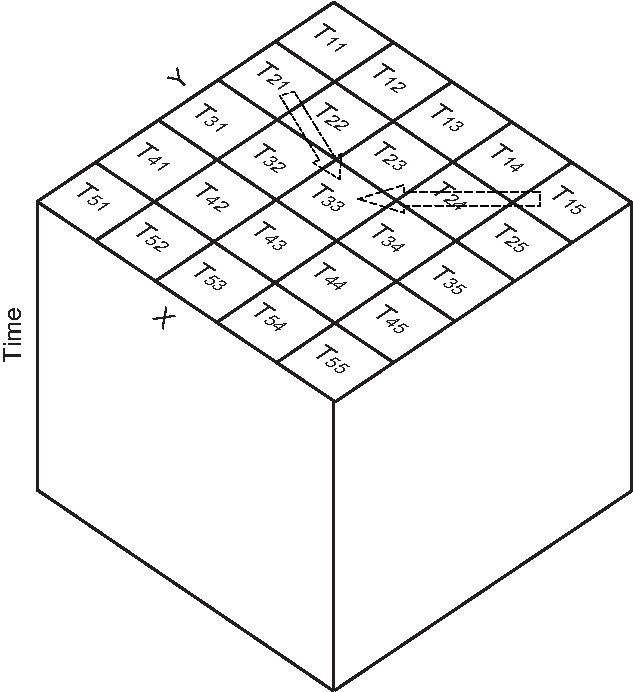
\includegraphics[height=2in]{plot/Fig/fig1}
  \end{figure}
\end{frame}

\begin{frame}
  \frametitle{\texttt{sfgraph}}
  \lstinputlisting[linerange=6-6]{plot/plot.sh}
  \begin{figure}
    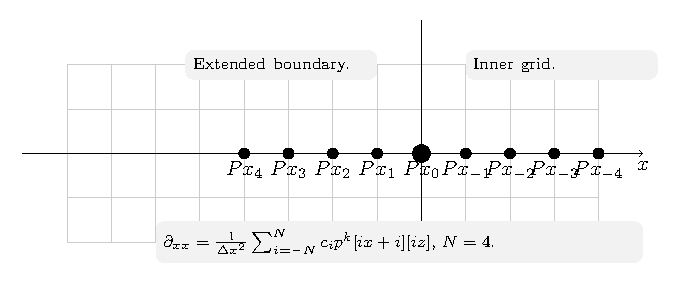
\includegraphics[height=2in]{plot/Fig/fig2}
  \end{figure}
\end{frame}

\begin{frame}
  \frametitle{\texttt{sfgraph}}
  \lstinputlisting[linerange=8-10]{plot/plot.sh}
  \begin{figure}
    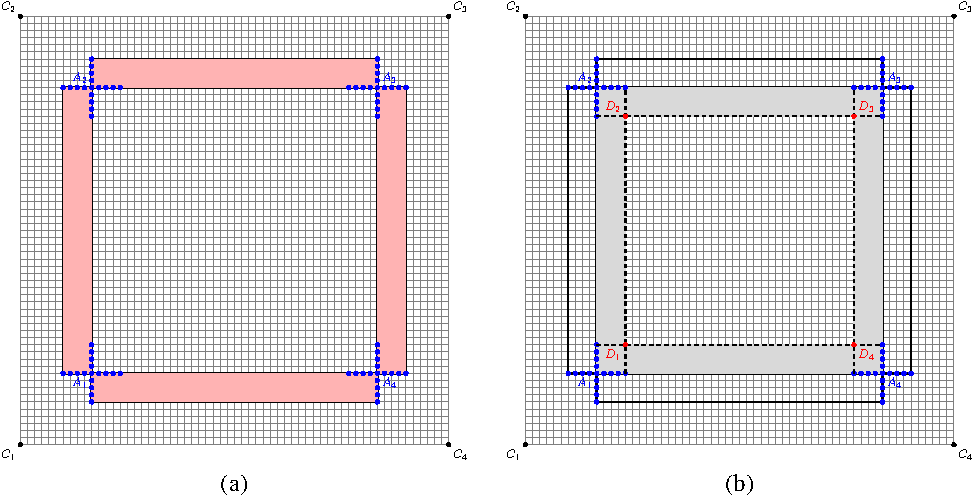
\includegraphics[height=2in]{plot/Fig/fig3}
  \end{figure}
\end{frame}

\begin{frame}
  \frametitle{\texttt{sfgraph}}
  \lstinputlisting[linerange=12-13]{plot/plot.sh}
  \begin{figure}
    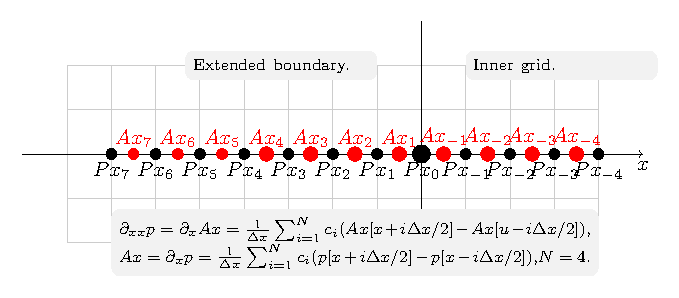
\includegraphics[height=2in]{plot/Fig/fig4}
  \end{figure}
\end{frame}

\begin{frame}
  \frametitle{\texttt{sfwiggle}}
  \lstinputlisting[linerange=25-25]{plot/plot.sh}
  \begin{figure}
    \includegraphics[height=2in]{plot/Fig/fig9}
  \end{figure}
\end{frame}

\begin{frame}
  \frametitle{\texttt{sfgrey}}
  \lstinputlisting[linerange=15-15]{plot/plot.sh}
  \begin{figure}
    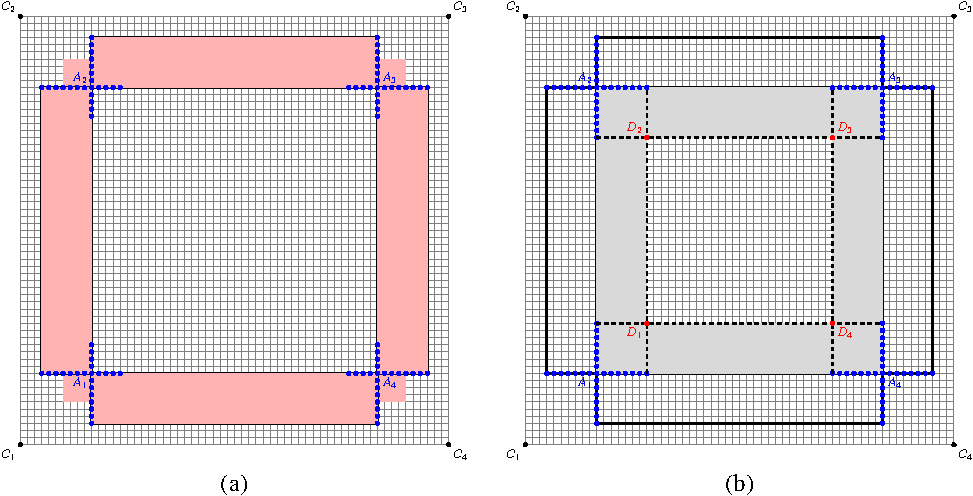
\includegraphics[height=2in]{plot/Fig/fig5}
  \end{figure}
\end{frame}

\begin{frame}
  \frametitle{\texttt{sfcontour}}
  \lstinputlisting[linerange=17-17]{plot/plot.sh}
  \begin{figure}
    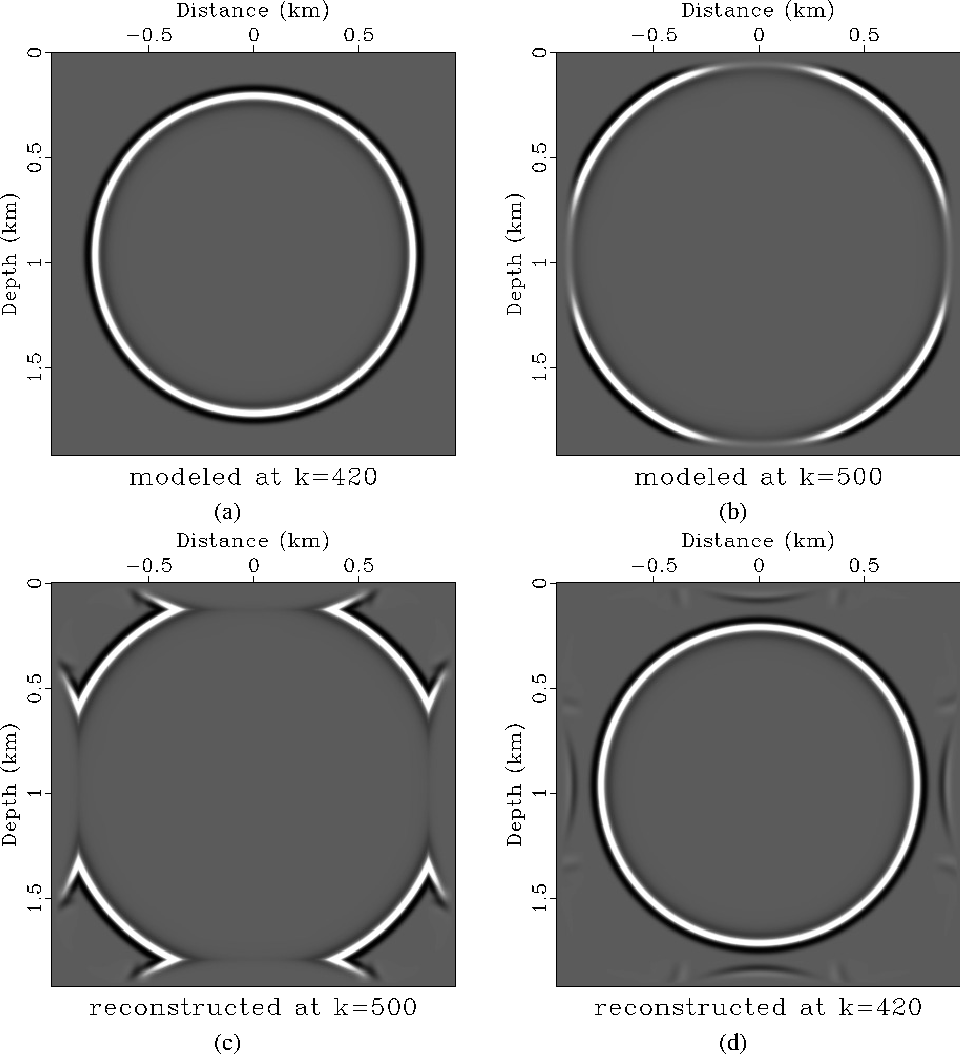
\includegraphics[height=2in]{plot/Fig/fig6}
  \end{figure}
\end{frame}

\begin{frame}
  \frametitle{Overlay}
  \lstinputlisting[linerange=19-21]{plot/plot.sh}
  \begin{figure}
    \includegraphics[height=2in]{plot/Fig/fig7}
  \end{figure}
\end{frame}

\begin{frame}
  \frametitle{\texttt{sfgrey3}}
  \lstinputlisting[linerange=23-23]{plot/plot.sh}
  \begin{figure}
    \includegraphics[height=2in]{plot/Fig/fig8}
  \end{figure}
\end{frame}

% \section{SAGE}

% \begin{frame}
%   \frametitle{SAGE}
%   \begin{itemize}
%     \item Collection of $100+$ packages
%     \item Interactive development environment
%     \item Notebook opened in web-browser
%     \item Based on Python
%   \end{itemize}
% \end{frame}

% \begin{frame}
%   \frametitle{SAGE interface to \textsc{Madagascar}}
% \end{frame}

\begin{frame}
  \begin{figure}
    \centering                                
    
\includegraphics[height=1.5in]{Fig/MadLogo}
  \end{figure}
  \begin{center}                                
    \Large{\url{http://www.ahay.org/}}
  \end{center}
\end{frame}

\begin{frame}
  \begin{center}                                
    \Large{Seismic Wave Analysis Group}
  \end{center}
    \begin{figure}
    \centering
    
\includegraphics[height=1.5in]{Fig/swag}
  \end{figure}
  \begin{center}                                
    \Large{\url{http://swag.kaust.edu.sa}}
  \end{center}
\end{frame}
